\documentclass[11pt]{article}
\usepackage[margin=1in]{geometry}
\usepackage[T1]{fontenc}
\usepackage{lmodern}
\usepackage{amsmath,amssymb,booktabs,graphicx,array}
\usepackage[round]{natbib}
\usepackage{placeins}
\usepackage[hidelinks]{hyperref}

% Result numbers. Generated by `crew.py numbers`; never typed by hand.
% Generated by `crew.py numbers` from claims.jsonl. Do not edit by hand.
% Each macro is a number taken from a logged run; see claims.jsonl.
\newcommand{\DidFte}{2.75}  % did-fte
\newcommand{\DidFteSe}{1.31}  % did-fte-se
\newcommand{\DidFteBalanced}{2.75}  % did-fte-balanced
\newcommand{\MeanWOnePa}{23.33}  % mean-w1-pa
\newcommand{\MeanWOnePaSe}{1.35}  % mean-w1-pa-se
\newcommand{\MeanWOneNj}{20.44}  % mean-w1-nj
\newcommand{\MeanWOneNjSe}{0.51}  % mean-w1-nj-se
\newcommand{\MeanWTwoPa}{21.17}  % mean-w2-pa
\newcommand{\MeanWTwoPaSe}{0.94}  % mean-w2-pa-se
\newcommand{\MeanWTwoNj}{21.03}  % mean-w2-nj
\newcommand{\MeanWTwoNjSe}{0.52}  % mean-w2-nj-se
\newcommand{\LevelGapWOne}{-2.89}  % level-gap-w1
\newcommand{\LevelGapWOneSe}{1.44}  % level-gap-w1-se
\newcommand{\LevelGapWTwo}{-0.14}  % level-gap-w2
\newcommand{\LevelGapWTwoSe}{1.08}  % level-gap-w2-se
\newcommand{\NWOnePa}{77}  % n-w1-pa
\newcommand{\NWTwoPa}{77}  % n-w2-pa
\newcommand{\NBalPa}{75}  % n-bal-pa
\newcommand{\NWOneNj}{321}  % n-w1-nj
\newcommand{\NWTwoNj}{319}  % n-w2-nj
\newcommand{\NBalNj}{309}  % n-bal-nj
\newcommand{\DidFtePa}{-2.17}  % did-fte-pa
\newcommand{\DidFtePaSe}{1.22}  % did-fte-pa-se
\newcommand{\DidFteNj}{0.59}  % did-fte-nj
\newcommand{\DidFteNjSe}{0.47}  % did-fte-nj-se
\newcommand{\DidFtePct}{13.5}  % did-fte-pct
\newcommand{\DidFteBalancedSe}{1.34}  % did-fte-balanced-se
\newcommand{\DidFteBalancedPa}{-2.28}  % did-fte-balanced-pa
\newcommand{\DidFteBalancedPaSe}{1.25}  % did-fte-balanced-pa-se
\newcommand{\DidFteBalancedNj}{0.47}  % did-fte-balanced-nj
\newcommand{\DidFteBalancedNjSe}{0.48}  % did-fte-balanced-nj-se
\newcommand{\DidFteBalancedPct}{13.5}  % did-fte-balanced-pct
\newcommand{\DidRFive}{2.51}  % did-r5
\newcommand{\DidRFiveSe}{1.35}  % did-r5-se
\newcommand{\HOneADidAbsdiff}{0.00639}  % h1a-did-absdiff
\newcommand{\HOneADidMet}{1}  % h1a-did-met
\newcommand{\HOneADidSeAbsdiff}{0.04997}  % h1a-did-se-absdiff
\newcommand{\HOneADidSeMet}{1}  % h1a-did-se-met
\newcommand{\HOneAPaAbsdiff}{0.00558}  % h1a-pa-absdiff
\newcommand{\HOneAPaMet}{1}  % h1a-pa-met
\newcommand{\HOneAPaSeAbsdiff}{0.02801}  % h1a-pa-se-absdiff
\newcommand{\HOneAPaSeMet}{1}  % h1a-pa-se-met
\newcommand{\HOneANjAbsdiff}{0.00198}  % h1a-nj-absdiff
\newcommand{\HOneANjMet}{1}  % h1a-nj-met
\newcommand{\HOneANjSeAbsdiff}{0.06786}  % h1a-nj-se-absdiff
\newcommand{\HOneANjSeMet}{0}  % h1a-nj-se-met
\newcommand{\HOneAPointMet}{1}  % h1a-point-met
\newcommand{\HOneASeMet}{0}  % h1a-se-met
\newcommand{\HOneAMet}{0}  % h1a-met
\newcommand{\HOneBDidAbsdiff}{0.00000}  % h1b-did-absdiff
\newcommand{\HOneBDidMet}{1}  % h1b-did-met
\newcommand{\HOneBDidSeAbsdiff}{0.00234}  % h1b-did-se-absdiff
\newcommand{\HOneBDidSeMet}{1}  % h1b-did-se-met
\newcommand{\HOneBPaAbsdiff}{0.00333}  % h1b-pa-absdiff
\newcommand{\HOneBPaMet}{1}  % h1b-pa-met
\newcommand{\HOneBPaSeAbsdiff}{0.00327}  % h1b-pa-se-absdiff
\newcommand{\HOneBPaSeMet}{1}  % h1b-pa-se-met
\newcommand{\HOneBNjAbsdiff}{0.00333}  % h1b-nj-absdiff
\newcommand{\HOneBNjMet}{1}  % h1b-nj-met
\newcommand{\HOneBNjSeAbsdiff}{0.00083}  % h1b-nj-se-absdiff
\newcommand{\HOneBNjSeMet}{1}  % h1b-nj-se-met
\newcommand{\HOneBPointMet}{1}  % h1b-point-met
\newcommand{\HOneBSeMet}{1}  % h1b-se-met
\newcommand{\HOneBMet}{1}  % h1b-met
\newcommand{\HOneCBNjAbsdiff}{0.00417}  % h1c-b-nj-absdiff
\newcommand{\HOneCBNjMet}{1}  % h1c-b-nj-met
\newcommand{\HOneCSeNjAbsdiff}{0.00160}  % h1c-se-nj-absdiff
\newcommand{\HOneCSeNjMet}{1}  % h1c-se-nj-met
\newcommand{\HOneCPointMet}{1}  % h1c-point-met
\newcommand{\HOneCSeMet}{1}  % h1c-se-met
\newcommand{\HOneCMet}{1}  % h1c-met
\newcommand{\HOneCNMet}{1}  % h1c-n-met
\newcommand{\RegN}{357}  % reg-n
\newcommand{\RegNNj}{290}  % reg-n-nj
\newcommand{\RegNPa}{67}  % reg-n-pa
\newcommand{\RegNj}{2.33}  % reg-nj
\newcommand{\RegNjSe}{1.19}  % reg-nj-se
\newcommand{\RegNjSeHcOne}{1.45}  % reg-nj-se-hc1
\newcommand{\RegRootMse}{8.79}  % reg-root-mse
\newcommand{\RegDepMean}{-0.24}  % reg-dep-mean
\newcommand{\RegDepSd}{8.83}  % reg-dep-sd
\newcommand{\SeClusterRThree}{1.31}  % se-cluster-r3
\newcommand{\SeClusterRFour}{1.34}  % se-cluster-r4
\newcommand{\SeHcOneRFour}{1.34}  % se-hc1-r4
\newcommand{\SeIndepPa}{1.65}  % se-indep-pa
\newcommand{\SeIndepNj}{0.73}  % se-indep-nj
\newcommand{\PlaceboHiwage}{0.13}  % placebo-hiwage
\newcommand{\PlaceboHiwageSe}{1.57}  % placebo-hiwage-se
\newcommand{\PlaceboHiwageNj}{-2.04}  % placebo-hiwage-nj
\newcommand{\PlaceboHiwageRFour}{0.13}  % placebo-hiwage-r4
\newcommand{\PlaceboHiwageRFourSe}{1.61}  % placebo-hiwage-r4-se
\newcommand{\PlaceboHiwageN}{71}  % placebo-hiwage-n
\newcommand{\HTwoN}{384}  % h2-n
\newcommand{\HTwoUnwinsorized}{2.75}  % h2-unwinsorized
\newcommand{\HTwoUnwinsorizedSe}{1.34}  % h2-unwinsorized-se
\newcommand{\HTwoWinsorized}{2.34}  % h2-winsorized
\newcommand{\HTwoWinsorizedSe}{1.10}  % h2-winsorized-se
\newcommand{\HTwoRatio}{0.85}  % h2-ratio
\newcommand{\HTwoQZeroFive}{-17.42}  % h2-q05
\newcommand{\HTwoQNineFive}{13.71}  % h2-q95
\newcommand{\HTwoCappedLowNj}{12}  % h2-capped-low-nj
\newcommand{\HTwoCappedLowPa}{8}  % h2-capped-low-pa
\newcommand{\HTwoCappedLowClosed}{1}  % h2-capped-low-closed
\newcommand{\HTwoCappedHighNj}{16}  % h2-capped-high-nj
\newcommand{\HTwoCappedHighPa}{4}  % h2-capped-high-pa
\newcommand{\HTwoCappedHighClosed}{0}  % h2-capped-high-closed
\newcommand{\HTwoFteOneBal}{21.0}  % h2-fte1-bal
\newcommand{\HTwoFteOneCappedLow}{46.0}  % h2-fte1-capped-low
\newcommand{\HTwoFteOneCappedHigh}{19.5}  % h2-fte1-capped-high
\newcommand{\HTwoSignSame}{1}  % h2-sign-same
\newcommand{\HTwoHalfKept}{1}  % h2-half-kept
\newcommand{\HTwoHolds}{1}  % h2-holds
\newcommand{\HTwoClosuresExcl}{2.33}  % h2-closures-excl
\newcommand{\HTwoClosuresExclSe}{1.09}  % h2-closures-excl-se
\newcommand{\HTwoClosuresExclRatio}{0.85}  % h2-closures-excl-ratio
\newcommand{\HTwoClosuresExclQZeroFive}{-17.07}  % h2-closures-excl-q05
\newcommand{\HTwoClosuresExclQNineFive}{13.79}  % h2-closures-excl-q95
\newcommand{\HTwoClosuresExclCappedLowNj}{12}  % h2-closures-excl-capped-low-nj
\newcommand{\HTwoClosuresExclCappedLowPa}{7}  % h2-closures-excl-capped-low-pa
\newcommand{\HTwoClosuresExclCappedHighNj}{15}  % h2-closures-excl-capped-high-nj
\newcommand{\HTwoClosuresExclCappedHighPa}{4}  % h2-closures-excl-capped-high-pa
\newcommand{\NwRuleDid}{2.78}  % nw-rule-did
\newcommand{\NwRuleDidSe}{1.16}  % nw-rule-did-se
\newcommand{\NwRuleDidSeHcOne}{1.34}  % nw-rule-did-se-hc1
\newcommand{\NwRuleN}{378}  % nw-rule-n
\newcommand{\NwRuleChgNj}{0.66}  % nw-rule-chg-nj
\newcommand{\NwRuleChgPa}{-2.06}  % nw-rule-chg-pa


\setlength{\emergencystretch}{2em}
\setlength{\belowcaptionskip}{6pt}
\renewcommand{\topfraction}{0.9}
\renewcommand{\bottomfraction}{0.8}
\renewcommand{\textfraction}{0.07}
\renewcommand{\floatpagefraction}{0.8}
\newcommand{\var}[1]{\texttt{#1}}

\title{Reproducing Card and Krueger (1994) from the Public Data:\\
A Logged Replication with a Tail-Winsorization Check}
\author{Bryce Wang (human PI) \\ \small Drafted with Free-Research-Crew; see the AI-use statement.}
\date{\today}

\begin{document}
\maketitle

\begin{abstract}
\noindent
We replicate the difference-in-differences estimates of \citet{card1994minimum} from the
authors' public data file, with the variable and sample rules of their own SAS program, and
with every target, tolerance and decision rule fixed before any analysis run. On the
balanced sample (Table~3, row~4) the New Jersey minus Pennsylvania difference in the change
in full-time-equivalent (FTE) employment per store is $\DidFteBalanced$ (SE
$\DidFteBalancedSe$), and every point and standard-error target of that row is reproduced.
Table~4, column~(i) is reproduced: on $\RegN$ stores the New Jersey coefficient is
$\RegNj$ ($\RegNjSe$); the count of $357$ is a data check, not a blind test. The headline
row~3 estimate, $\DidFte$ against the published $2.76$, is within the pre-registered
tolerance but not at published precision: the gap lies in the unbalanced wave means, is not
rounding, and its source is unidentified. For the row-3 standard errors the verdict is
``point reproduced; SE construction not identified''. Winsorizing store-level changes at the
pooled 5th and 95th percentiles leaves $\HTwoWinsorized$ of the balanced-sample
$\HTwoUnwinsorized$ (ratio $\HTwoRatio$), so our second hypothesis holds; this is a check
on the tails only and does not answer Neumark and Wascher's broader measurement-error
critique. With one treated and one control state, all standard errors here are cross-store
sampling errors, and we draw no design-based inference from them.
\end{abstract}

\section{Introduction}

On April~1, 1992, New Jersey raised its minimum wage from \$4.25 to \$5.05 an hour.
\citet{card1994minimum} surveyed 410 fast-food restaurants in New Jersey and eastern
Pennsylvania in February--March 1992, before the rise, and again in November--December 1992,
after it. Relative to Pennsylvania, mean full-time-equivalent (FTE) employment per store
rose in New Jersey by 2.76 (standard error 1.36), about 13 percent
\citep[Table~3, row~3]{card1994minimum}. The estimate was contested. Using payroll records from restaurants in the same area,
\citet{neumark1995payroll} estimate that the increase reduced New Jersey employment by
4.6 percent relative to Pennsylvania, and report that the standard deviation of employment
changes in the survey data is about three times that in the payroll data.
\citet{card1998reanalysis}, using BLS ES-202 payroll records, find similar or slightly
faster employment growth in New Jersey, and attribute the Neumark--Wascher result to the
Pennsylvania restaurants of a single franchisee and to differences in reporting intervals.

This paper does not take a side in that dispute; neither payroll data set is public.
It asks two narrower questions that the public survey data can answer.

The first is whether the published estimates can be reproduced from the authors' public
file, including the parts that earlier replications missed. An informal replication from
the same file reproduces the Table~3 means and a difference-in-differences of 2.75, but not
the published standard errors or the 357-store regression sample of Table~4
\citep{mamula2021replicating}. A 2025 preprint, whose data source is not stated, reports 3.36
and 3.44 where the paper has 2.76 and 2.75, and no Table~4 sample size
\citep{morshed2025replication}. Our hypothesis H1 sets numeric targets for
Table~3 rows~3 and~4 and Table~4 column~(i), points and standard errors alike, with a
tolerance of $0.05$ fixed before any estimate was computed.

The second is how much of the balanced-sample estimate remains when the extreme store-level
changes that \citet{neumark1995payroll} point to are capped. We found no published
winsorized or trimmed estimate on these data. The distributional question itself has been
asked: with a changes-in-changes estimator, \citet{ropponen2010cic} reports an average
effect of 0.90 FTE against a difference-in-differences of 2.72 on the same 376 stores, with
positive effects at small restaurants and negative effects at large ones. Our hypothesis H2
winsorizes the store-level changes at the pooled 5th and 95th percentiles and asks whether
the estimate keeps its sign and at least half its size.

The answers are as follows.
\begin{itemize}
  \item \textbf{H1(b), Table~3 row~4 (balanced sample): reproduced.} The difference is
        $\DidFteBalanced$ ($\DidFteBalancedSe$) against the published 2.75 (1.34), and all
        six point and standard-error targets are met.
  \item \textbf{H1(c), Table~4 column~(i): reproduced.} With the sample rule of the
        authors' SAS program, the regression has $\RegN$ stores and a New Jersey
        coefficient of $\RegNj$ ($\RegNjSe$) against the published 2.33 (1.19). The store
        count was already observed at data preparation, so $N = 357$ is a data check, not a
        blind test.
  \item \textbf{H1(a), Table~3 row~3 (the headline): not reproduced as a whole.} The three
        point estimates are within the tolerance but not at published precision. The
        difference is $\DidFte$ against 2.76; the gap lies in the unbalanced wave means, it
        is not rounding, and its source is unidentified. For the standard errors, the
        verdict is ``point reproduced; SE construction not identified''.
  \item \textbf{H2: holds.} Winsorized, the balanced-sample difference is
        $\HTwoWinsorized$ against $\HTwoUnwinsorized$ unwinsorized, a ratio of
        $\HTwoRatio$. The check caps only the tails. It does not answer Neumark and
        Wascher's broader critique that the survey's extra variability is not driven by a
        few outliers \citep{neumark1995payroll}.
\end{itemize}
Under Neumark and Wascher's own sample rule we obtain $\NwRuleDid$, the value they report;
their sample size is not recorded in our sources, so we do not claim the samples coincide.

Two features of the process matter for reading these results. First, every planned analysis run was
listed, with its metrics and decision rule, in a plan approved by the human author before
any analysis run; the code was reviewed before any analysis run; and each executed once.
Four presentation runs that build the tables and the figure from the logged metrics were
added after the results gate and compute no new estimate
(Section~\ref{sec:deviations}), which also discloses that the design gate preceded the code
review. What
this rules out is specification search within this study. It does not make the study
blind: the crew had read the published results of Card and Krueger's and Neumark and
Wascher's robustness checks and of the earlier replications before choosing the
hypotheses. Second, with one treated and one control state, the standard errors of the
original paper and of this replication are cross-store sampling errors that cannot be
clustered at the level of treatment \citep{conley2011inference}. We report them only to
compare with the published ones (Section~\ref{sec:inference}).

Section~\ref{sec:original} describes the original study and the later debate,
Section~\ref{sec:data} the data, Section~\ref{sec:impl} our implementation and decision
rules, and Section~\ref{sec:results} the results. Sections~\ref{sec:inference}
to~\ref{sec:deviations} discuss inference, limitations, and deviations and disclosures.

\section{The original study}
\label{sec:original}

\paragraph{Design.} \citet{card1994minimum} surveyed restaurants of four chains (Burger
King, KFC, Wendy's and Roy Rogers) in New Jersey and eastern Pennsylvania, where the
minimum wage stayed at \$4.25. The first wave ran from February~15 to March~4, 1992, and the
second from November~5 to December~31, 1992; only first-wave respondents were contacted in
the second wave. FTE employment is the number of full-time workers, including managers and
assistant managers, plus 0.5 times the number of part-time workers
\citep[p.~775 and Table~5 notes]{card1994minimum}. In Table~3, second-wave employment is
set to zero at the six permanently closed stores and treated as missing at the four
temporarily closed stores \citep{card1994minimum}.

\paragraph{Published estimates.} Mean FTE employment per store fell from 23.33 to 21.17 in
Pennsylvania and rose from 20.44 to 21.03 in New Jersey \citep[Table~3, rows~1--2]{card1994minimum}.
Row~3, ``change in mean FTE employment'', uses all stores with employment data in a wave and
gives a New Jersey minus Pennsylvania difference of 2.76 (1.36), with a $t$ statistic of
2.03. Row~4 restricts to the balanced sample of stores with employment data in both waves
and gives 2.75 (1.34); row~5, which also sets the temporarily closed stores to zero, gives
2.51 (1.35). Table~4 regresses the change in FTE employment on a New Jersey dummy for 357
stores with employment and starting-wage data in both waves: the coefficient is 2.33 (1.19)
without controls and 2.30 (1.20) with chain and ownership controls. Within New Jersey,
stores that initially paid \$4.25 gained 3.36 (1.48) FTE more than stores that paid
\$5.00 or more \citep[Table~3]{card1994minimum}. The published targets of this replication
are collected in Table~\ref{tab:replication}.

\paragraph{What the paper does not document.} The paper does not say how the Table~3
standard errors were computed. Two facts constrain them, both arithmetic on the published
entries. The column~(iii) standard errors equal $\sqrt{SE_{PA}^2 + SE_{NJ}^2}$, which treats
the two states as independent samples. And the Pennsylvania change has a standard error of
1.25, below the $\sqrt{1.35^2 + 0.94^2} = 1.64$ that independent waves would give, so the
within-state errors allow for the correlation between a store's two waves. Nothing in the
paper pins down how they handle stores observed in only one wave.

\paragraph{The later debate.} Using payroll records, \citet{neumark1995payroll} estimate a
4.6 percent relative decline in New Jersey employment, an elasticity of $-0.24$. On Card and
Krueger's survey data, excluding closed stores and controlling for chain and ownership, they
obtain a difference-in-differences of 2.78. They also state that the greater variability of
employment changes in the survey data is not driven by one or two outliers: the standard
deviation of the change is 9.6 in the survey data against 3.2 in the payroll data.
\citet{card1998reanalysis} answer with BLS ES-202 records, as described in the
introduction. The exchange was published as \citet{neumark2000comment} and
\citet{card2000reply}; we could not read their full texts and cite them for their
existence only.

\paragraph{Reanalyses of the public data.} \citet{ropponen2010cic} applies changes-in-changes
to 301 New Jersey and 75 Pennsylvania stores (eight New Jersey stores fall outside the
support of the Pennsylvania distribution and are dropped). He reports an average effect of
0.90 FTE (bootstrap SE 0.44) against a difference-in-differences of 2.72 on the same 376
stores, and effects that are positive for small and negative for large restaurants. Because
the 2.72 is on 376 stores, not on the 384-store balanced sample, it is not a replication of
the published 2.75. Applying the same estimator to both the Card--Krueger and the
Neumark--Wascher data, \citet{ropponen2011reconciling} concludes that the positive result
holds only for small restaurants; with Abadie's semiparametric difference-in-differences,
\citet{ropponen2014note} finds the overall effects fairly robust. The informal replication from the public file does not reproduce the published standard
errors or the 357-store sample \citep{mamula2021replicating}. The 2025 preprint, whose data
source is not stated, reports point estimates far from the published ones and no Table~4
sample size \citep{morshed2025replication}; neither replication reproduces the published
standard errors.

\section{Data}
\label{sec:data}

\paragraph{Source.} The authors' archive \texttt{njmin.zip} contains \texttt{public.dat}
(410 observations), a codebook, a SAS program for key tabulations (\texttt{check.sas}), and
the texts of both survey questionnaires \citep{card_njmin_readme}. Its readme says the files
pertain to the surveys used in chapter~2 of Card and Krueger's book \emph{Myth and
Measurement}, not to the 1994 article, so the public file may differ from the one behind the
published tables. We fetched the archive on 2026-11-19 from
\url{https://davidcard.berkeley.edu/data_sets/njmin.zip} (23{,}017 bytes; its SHA-256 is
pinned in the workspace's data manifest, so a rerun gets the same bytes or fails). No terms
of use are stated; the raw and derived files are not redistributed and are rebuilt by the
logged data-preparation runs.

\paragraph{Parsing and checks.} We read \texttt{public.dat} at the column positions in the
codebook; reading it as \texttt{check.sas} does, with whitespace-separated list input, gives
identical values on all 410 rows. The file has 331 New Jersey and 79 Pennsylvania stores, as
in Card and Krueger's Table~1, and the counts of second-wave interviews (321 and 78),
closures and refusals equal those of the codebook and the paper. In New Jersey, 101, 140 and
73 stores have a first-wave starting wage of \$4.25, between \$4.26 and \$4.99, and \$5.00 or
more, the group sizes printed in Table~3. These are counts of stores; no statistic relating
the state to employment was computed before the design gate.

\paragraph{Store key: SHEET 407.} The codebook calls the variable \var{SHEET} a ``unique
store id'', but \var{SHEET}~$=407$ appears twice, on two different stores: a Pennsylvania KFC
(line 42 of \texttt{public.dat}) and a New Jersey Wendy's (line 168). We therefore key
stores by their line number, \var{ROW\_ID} (1--410), and use \var{SHEET} only as a label. No
estimate in this paper merges or clusters on \var{SHEET}, so the duplicate does not affect
the estimates, but a replication that clustered or merged on it would mislabel one store.
The file has no store address and no first-wave interview date, so it cannot be linked to
other data.

\paragraph{Closures.} The second-wave status variable \var{STATUS2} records six permanent
closures (five in New Jersey, one in Pennsylvania), four temporary closures, all in New
Jersey (two for renovation, one for highway construction, one after a mall fire), and one
New Jersey refusal. The raw file already codes all three employment components as zero at
the permanent closures, and leaves second-wave employment missing at the temporary closures
and the refusal. One store closed for renovation (line 198) reports some second-wave items,
the number of managers and the starting wage, but not full-time or part-time employment, so
its second-wave FTE is missing, as in the paper.

\paragraph{Variables.} Employment is reported in three parts in each wave: full-time
workers excluding managers (\var{EMPFT}), part-time workers excluding managers
(\var{EMPPT}), and managers and assistant managers (\var{NMGRS}); the questionnaire wording
confirms that managers are counted only in the third. The other variables we use are the
state, the chain, a company-ownership dummy (\var{CO\_OWNED}), the first- and second-wave
starting wages (\var{WAGE\_ST}, \var{WAGE\_ST2}) and \var{STATUS2}.

\section{Our implementation}
\label{sec:impl}

All rules in this section were fixed in the plan approved at the design gate, before any
analysis run.

\subsection{Variables and samples}

FTE employment follows the authors' \texttt{check.sas} (its \var{EMPTOT}):
\begin{equation*}
  \text{FTE}_1 = \var{EMPFT} + \var{NMGRS} + 0.5\,\var{EMPPT}, \qquad
  \text{FTE}_2 = \var{EMPFT2} + \var{NMGRS2} + 0.5\,\var{EMPPT2},
\end{equation*}
missing if any part is missing, as in SAS. After construction a closure override is applied
whatever the raw components say: $\text{FTE}_2 = 0$ at the six permanent closures, and
missing at the four temporary closures and the refusal (zero only in the report-only row~5).
The code also asserts that the raw file already agrees with the override, and stops if it
does not. The store-level change is $\Delta\text{FTE} = \text{FTE}_2 - \text{FTE}_1$.

The samples are:
\begin{itemize}
  \item \emph{Rows 1--3} (unbalanced): first-wave means over all stores with
        $\text{FTE}_1$, second-wave means over all stores with $\text{FTE}_2$:
        $\NWOnePa$ and $\NWTwoPa$ Pennsylvania stores, $\NWOneNj$ and $\NWTwoNj$ New Jersey
        stores. Row~3 is row~2 minus row~1.
  \item \emph{Row 4} (balanced, sample $B$): stores with both $\text{FTE}_1$ and
        $\text{FTE}_2$, $\NBalPa$ in Pennsylvania and $\NBalNj$ in New Jersey, with the
        permanent closures in it at $\text{FTE}_2 = 0$.
  \item \emph{Row 5} (report only): $B$ plus the temporarily closed stores at
        $\text{FTE}_2 = 0$.
  \item \emph{Table 4} (the \texttt{check.sas} data step \texttt{C1}, verbatim):
        $\Delta\text{FTE}$ non-missing, and either the store closed permanently or both
        starting wages are present. This gives $\RegN$ stores ($\RegNNj$ New Jersey,
        $\RegNPa$ Pennsylvania).
\end{itemize}

\subsection{Estimators and standard errors}

\paragraph{Table 3 (method S1).} For state $s$, let $A_1$ be the $n_1$ stores with
$\text{FTE}_1$, $A_2$ the $n_2$ stores with $\text{FTE}_2$, and $A_{12}$ the $n_{12}$ stores
with both. The change is $\widehat\Delta_s = \overline{\text{FTE}}_{2,A_2} -
\overline{\text{FTE}}_{1,A_1}$, with variance
\begin{equation*}
  \widehat V(\widehat\Delta_s) = \frac{s_1^2}{n_1} + \frac{s_2^2}{n_2}
     - \frac{2\,c_{12}\,n_{12}}{n_1 n_2},
\end{equation*}
where $s_1^2$ and $s_2^2$ are the sample variances of $\text{FTE}_1$ on $A_1$ and
$\text{FTE}_2$ on $A_2$, and $c_{12}$ is the sample covariance of the two on $A_{12}$. On a
balanced sample this reduces to $\mathrm{sd}(\Delta\text{FTE})^2/n$, the HC2 variance of a
regression of $\Delta\text{FTE}$ on a New Jersey dummy. The difference-in-differences is
$\widehat\Delta_{NJ} - \widehat\Delta_{PA}$, with standard error
$\sqrt{SE_{PA}^2 + SE_{NJ}^2}$.

S1 is \emph{our reconstruction}, not a documented method. We chose it because it is
consistent with the two facts about the published standard errors in
Section~\ref{sec:original}, both of which come from the Pennsylvania entries and the
column~(iii) combination. Before any run, the Reviewer showed that the New Jersey entries do
not single it out: if the variances inside and outside the balanced panel are equal, S1
implies about 0.48 for the row-3 New Jersey change, not the published 0.54. The plan
therefore fixed the wording of both outcomes in advance: a match would be reported as ``S1
reproduces the published standard errors'', never as Card and Krueger's method; a miss with
the points met would be reported as ``point reproduced; SE construction not identified''.

\paragraph{Table 4.} OLS of $\Delta\text{FTE}_i$ on a constant and a New Jersey dummy, with
the conventional homoskedastic standard error that SAS \texttt{PROC REG}, used by
\texttt{check.sas}, reports. The HC1 standard error is reported only.

\paragraph{Alternative standard errors (report only).} A stacked store-by-wave regression
$\text{FTE}_{it} = a + b\,NJ_i + c\,\text{Post}_t + d\,NJ_i\text{Post}_t$ with standard errors
clustered by store (CR1) on the row-3 and row-4 samples; the HC1 and HC2 standard errors of
the change regression on $B$; and the independent-waves standard error
$\sqrt{s_1^2/n_1 + s_2^2/n_2}$ of each row-3 change. None of these was used for a verdict.

\subsection{Decision rules}

\paragraph{H1.} The targets are the published Table~3 row~3 (H1(a): 2.76 (1.36), with
Pennsylvania $-2.16$ (1.25) and New Jersey 0.59 (0.54)), row~4 (H1(b): 2.75 (1.34),
$-2.28$ (1.25), 0.47 (0.48)) and Table~4 column~(i) (H1(c): $N = 357$ exactly, coefficient
2.33 (1.19)). A target is met if the absolute difference between the unrounded replicated
value and the published value is at most $0.05$, after rounding the difference to six
decimals. A part is reproduced only if all its targets are met; point and standard-error
targets are also reported separately. The tolerance allows for rounding and for differences
between data releases. The within-state targets are included because the two difference
estimates lie within the tolerance of each other, while the New Jersey changes (0.59 against
0.47) separate the row-3 and row-4 sample rules.

\paragraph{H2.} On sample $B$, with the permanent closures at $\Delta\text{FTE} =
-\text{FTE}_1$, let $q_{05}$ and $q_{95}$ be the 5th and 95th percentiles of
$\Delta\text{FTE}$ over all stores of both states, closures included (linear
interpolation). The winsorized change is $W_i = \min(\max(\Delta\text{FTE}_i, q_{05}),
q_{95})$, and a store counts as capped only if it lies strictly beyond a cutoff. H2 holds if
$\overline W_{NJ} - \overline W_{PA}$ has the sign of the unwinsorized difference on the
same stores and at least half its magnitude, judged on unrounded point estimates, not on
significance. Two secondaries are reported but not judged: (s1) the six permanent closures
are left out of the percentile pool and never capped; (s2) the Neumark--Wascher rule,
sample $B$ without the permanent closures and OLS of $\Delta\text{FTE}$ on the New Jersey
dummy, chain dummies and company ownership.

\paragraph{One judge.} A single script reads the logged metrics and writes, for each H1
target, the published value, the absolute difference and a met flag, and the H2 flags. No
hypothesis is judged anywhere else, and every number in this paper is generated from the
logged runs.

\subsection{Verification before and after the runs}

After the design gate and before any analysis run, the code was written and a test script
ran every estimator on a synthetic file shaped like
the public one (closures, item non-response, a duplicated \var{SHEET}) and checked, among
other things, that S1 equals HC2 on a balanced sample, that the stacked regression
reproduces the difference of state mean changes, that winsorization caps exactly the stores
beyond the cutoffs, and that the Table~4 filter equals a literal transcription of
\texttt{check.sas} on hand-built cases. The Reviewer then reviewed the code against the plan
and \texttt{check.sas}; its three minor findings (binding the run script to the reviewed
code by hash, removing the option to overwrite a run, and testing the values of the
report-only estimators) were fixed before any analysis run. The eight analysis runs then
executed once each, in the planned order, on the reviewed code. At the results review the
Reviewer re-implemented every estimator from the raw file without our code and matched every
metric to $10^{-12}$. The software is Python with pandas, NumPy and statsmodels, at the
versions pinned in the workspace; all estimators are deterministic.

\section{Results}
\label{sec:results}

\begin{table}[tbp]
\centering
\caption{Published and replicated estimates of \citet{card1994minimum}, Table~3 rows~1--5
and Table~4 column~(i). The replication uses the authors' public file (410 stores) and the
sample and variable rules of their \texttt{check.sas}.}
\label{tab:replication}
{\footnotesize\resizebox{\textwidth}{!}{% Generated by code/tab_replication.py from logged runs. Do not edit by hand; rerun the script.
% Needs \usepackage{booktabs} and % Generated by `crew.py numbers` from claims.jsonl. Do not edit by hand.
% Each macro is a number taken from a logged run; see claims.jsonl.
\newcommand{\DidFte}{2.75}  % did-fte
\newcommand{\DidFteSe}{1.31}  % did-fte-se
\newcommand{\DidFteBalanced}{2.75}  % did-fte-balanced
\newcommand{\MeanWOnePa}{23.33}  % mean-w1-pa
\newcommand{\MeanWOnePaSe}{1.35}  % mean-w1-pa-se
\newcommand{\MeanWOneNj}{20.44}  % mean-w1-nj
\newcommand{\MeanWOneNjSe}{0.51}  % mean-w1-nj-se
\newcommand{\MeanWTwoPa}{21.17}  % mean-w2-pa
\newcommand{\MeanWTwoPaSe}{0.94}  % mean-w2-pa-se
\newcommand{\MeanWTwoNj}{21.03}  % mean-w2-nj
\newcommand{\MeanWTwoNjSe}{0.52}  % mean-w2-nj-se
\newcommand{\LevelGapWOne}{-2.89}  % level-gap-w1
\newcommand{\LevelGapWOneSe}{1.44}  % level-gap-w1-se
\newcommand{\LevelGapWTwo}{-0.14}  % level-gap-w2
\newcommand{\LevelGapWTwoSe}{1.08}  % level-gap-w2-se
\newcommand{\NWOnePa}{77}  % n-w1-pa
\newcommand{\NWTwoPa}{77}  % n-w2-pa
\newcommand{\NBalPa}{75}  % n-bal-pa
\newcommand{\NWOneNj}{321}  % n-w1-nj
\newcommand{\NWTwoNj}{319}  % n-w2-nj
\newcommand{\NBalNj}{309}  % n-bal-nj
\newcommand{\DidFtePa}{-2.17}  % did-fte-pa
\newcommand{\DidFtePaSe}{1.22}  % did-fte-pa-se
\newcommand{\DidFteNj}{0.59}  % did-fte-nj
\newcommand{\DidFteNjSe}{0.47}  % did-fte-nj-se
\newcommand{\DidFtePct}{13.5}  % did-fte-pct
\newcommand{\DidFteBalancedSe}{1.34}  % did-fte-balanced-se
\newcommand{\DidFteBalancedPa}{-2.28}  % did-fte-balanced-pa
\newcommand{\DidFteBalancedPaSe}{1.25}  % did-fte-balanced-pa-se
\newcommand{\DidFteBalancedNj}{0.47}  % did-fte-balanced-nj
\newcommand{\DidFteBalancedNjSe}{0.48}  % did-fte-balanced-nj-se
\newcommand{\DidFteBalancedPct}{13.5}  % did-fte-balanced-pct
\newcommand{\DidRFive}{2.51}  % did-r5
\newcommand{\DidRFiveSe}{1.35}  % did-r5-se
\newcommand{\HOneADidAbsdiff}{0.00639}  % h1a-did-absdiff
\newcommand{\HOneADidMet}{1}  % h1a-did-met
\newcommand{\HOneADidSeAbsdiff}{0.04997}  % h1a-did-se-absdiff
\newcommand{\HOneADidSeMet}{1}  % h1a-did-se-met
\newcommand{\HOneAPaAbsdiff}{0.00558}  % h1a-pa-absdiff
\newcommand{\HOneAPaMet}{1}  % h1a-pa-met
\newcommand{\HOneAPaSeAbsdiff}{0.02801}  % h1a-pa-se-absdiff
\newcommand{\HOneAPaSeMet}{1}  % h1a-pa-se-met
\newcommand{\HOneANjAbsdiff}{0.00198}  % h1a-nj-absdiff
\newcommand{\HOneANjMet}{1}  % h1a-nj-met
\newcommand{\HOneANjSeAbsdiff}{0.06786}  % h1a-nj-se-absdiff
\newcommand{\HOneANjSeMet}{0}  % h1a-nj-se-met
\newcommand{\HOneAPointMet}{1}  % h1a-point-met
\newcommand{\HOneASeMet}{0}  % h1a-se-met
\newcommand{\HOneAMet}{0}  % h1a-met
\newcommand{\HOneBDidAbsdiff}{0.00000}  % h1b-did-absdiff
\newcommand{\HOneBDidMet}{1}  % h1b-did-met
\newcommand{\HOneBDidSeAbsdiff}{0.00234}  % h1b-did-se-absdiff
\newcommand{\HOneBDidSeMet}{1}  % h1b-did-se-met
\newcommand{\HOneBPaAbsdiff}{0.00333}  % h1b-pa-absdiff
\newcommand{\HOneBPaMet}{1}  % h1b-pa-met
\newcommand{\HOneBPaSeAbsdiff}{0.00327}  % h1b-pa-se-absdiff
\newcommand{\HOneBPaSeMet}{1}  % h1b-pa-se-met
\newcommand{\HOneBNjAbsdiff}{0.00333}  % h1b-nj-absdiff
\newcommand{\HOneBNjMet}{1}  % h1b-nj-met
\newcommand{\HOneBNjSeAbsdiff}{0.00083}  % h1b-nj-se-absdiff
\newcommand{\HOneBNjSeMet}{1}  % h1b-nj-se-met
\newcommand{\HOneBPointMet}{1}  % h1b-point-met
\newcommand{\HOneBSeMet}{1}  % h1b-se-met
\newcommand{\HOneBMet}{1}  % h1b-met
\newcommand{\HOneCBNjAbsdiff}{0.00417}  % h1c-b-nj-absdiff
\newcommand{\HOneCBNjMet}{1}  % h1c-b-nj-met
\newcommand{\HOneCSeNjAbsdiff}{0.00160}  % h1c-se-nj-absdiff
\newcommand{\HOneCSeNjMet}{1}  % h1c-se-nj-met
\newcommand{\HOneCPointMet}{1}  % h1c-point-met
\newcommand{\HOneCSeMet}{1}  % h1c-se-met
\newcommand{\HOneCMet}{1}  % h1c-met
\newcommand{\HOneCNMet}{1}  % h1c-n-met
\newcommand{\RegN}{357}  % reg-n
\newcommand{\RegNNj}{290}  % reg-n-nj
\newcommand{\RegNPa}{67}  % reg-n-pa
\newcommand{\RegNj}{2.33}  % reg-nj
\newcommand{\RegNjSe}{1.19}  % reg-nj-se
\newcommand{\RegNjSeHcOne}{1.45}  % reg-nj-se-hc1
\newcommand{\RegRootMse}{8.79}  % reg-root-mse
\newcommand{\RegDepMean}{-0.24}  % reg-dep-mean
\newcommand{\RegDepSd}{8.83}  % reg-dep-sd
\newcommand{\SeClusterRThree}{1.31}  % se-cluster-r3
\newcommand{\SeClusterRFour}{1.34}  % se-cluster-r4
\newcommand{\SeHcOneRFour}{1.34}  % se-hc1-r4
\newcommand{\SeIndepPa}{1.65}  % se-indep-pa
\newcommand{\SeIndepNj}{0.73}  % se-indep-nj
\newcommand{\PlaceboHiwage}{0.13}  % placebo-hiwage
\newcommand{\PlaceboHiwageSe}{1.57}  % placebo-hiwage-se
\newcommand{\PlaceboHiwageNj}{-2.04}  % placebo-hiwage-nj
\newcommand{\PlaceboHiwageRFour}{0.13}  % placebo-hiwage-r4
\newcommand{\PlaceboHiwageRFourSe}{1.61}  % placebo-hiwage-r4-se
\newcommand{\PlaceboHiwageN}{71}  % placebo-hiwage-n
\newcommand{\HTwoN}{384}  % h2-n
\newcommand{\HTwoUnwinsorized}{2.75}  % h2-unwinsorized
\newcommand{\HTwoUnwinsorizedSe}{1.34}  % h2-unwinsorized-se
\newcommand{\HTwoWinsorized}{2.34}  % h2-winsorized
\newcommand{\HTwoWinsorizedSe}{1.10}  % h2-winsorized-se
\newcommand{\HTwoRatio}{0.85}  % h2-ratio
\newcommand{\HTwoQZeroFive}{-17.42}  % h2-q05
\newcommand{\HTwoQNineFive}{13.71}  % h2-q95
\newcommand{\HTwoCappedLowNj}{12}  % h2-capped-low-nj
\newcommand{\HTwoCappedLowPa}{8}  % h2-capped-low-pa
\newcommand{\HTwoCappedLowClosed}{1}  % h2-capped-low-closed
\newcommand{\HTwoCappedHighNj}{16}  % h2-capped-high-nj
\newcommand{\HTwoCappedHighPa}{4}  % h2-capped-high-pa
\newcommand{\HTwoCappedHighClosed}{0}  % h2-capped-high-closed
\newcommand{\HTwoFteOneBal}{21.0}  % h2-fte1-bal
\newcommand{\HTwoFteOneCappedLow}{46.0}  % h2-fte1-capped-low
\newcommand{\HTwoFteOneCappedHigh}{19.5}  % h2-fte1-capped-high
\newcommand{\HTwoSignSame}{1}  % h2-sign-same
\newcommand{\HTwoHalfKept}{1}  % h2-half-kept
\newcommand{\HTwoHolds}{1}  % h2-holds
\newcommand{\HTwoClosuresExcl}{2.33}  % h2-closures-excl
\newcommand{\HTwoClosuresExclSe}{1.09}  % h2-closures-excl-se
\newcommand{\HTwoClosuresExclRatio}{0.85}  % h2-closures-excl-ratio
\newcommand{\HTwoClosuresExclQZeroFive}{-17.07}  % h2-closures-excl-q05
\newcommand{\HTwoClosuresExclQNineFive}{13.79}  % h2-closures-excl-q95
\newcommand{\HTwoClosuresExclCappedLowNj}{12}  % h2-closures-excl-capped-low-nj
\newcommand{\HTwoClosuresExclCappedLowPa}{7}  % h2-closures-excl-capped-low-pa
\newcommand{\HTwoClosuresExclCappedHighNj}{15}  % h2-closures-excl-capped-high-nj
\newcommand{\HTwoClosuresExclCappedHighPa}{4}  % h2-closures-excl-capped-high-pa
\newcommand{\NwRuleDid}{2.78}  % nw-rule-did
\newcommand{\NwRuleDidSe}{1.16}  % nw-rule-did-se
\newcommand{\NwRuleDidSeHcOne}{1.34}  % nw-rule-did-se-hc1
\newcommand{\NwRuleN}{378}  % nw-rule-n
\newcommand{\NwRuleChgNj}{0.66}  % nw-rule-chg-nj
\newcommand{\NwRuleChgPa}{-2.06}  % nw-rule-chg-pa
 for the macros.
\begin{tabular}{@{}ll rrrrl rrrrl@{}}
\toprule
 & & \multicolumn{5}{c}{Estimate} & \multicolumn{5}{c}{Standard error} \\
\cmidrule(lr){3-7}\cmidrule(lr){8-12}
Row & Column & Publ. & Repl. & $|\Delta|$ & Tol. & Status & Publ. & Repl. & $|\Delta|$ & Tol. & Status \\
\midrule
\multicolumn{12}{@{}l}{\textit{Table 3: mean FTE employment per store}} \\
1.\ Wave 1, all available & PA & $23.33$ & $\MeanWOnePa$ & $0.00117$ & -- & report only & $1.35$ & $\MeanWOnePaSe$ & $0.00115$ & -- & report only \\
 & NJ & $20.44$ & $\MeanWOneNj$ & $0.00059$ & -- & report only & $0.51$ & $\MeanWOneNjSe$ & $0.00174$ & -- & report only \\
 & NJ $-$ PA & $-2.89$ & $\LevelGapWOne$ & $0.00176$ & -- & report only & $1.44$ & $\LevelGapWOneSe$ & $0.00358$ & -- & report only \\
\addlinespace
2.\ Wave 2, all available & PA & $21.17$ & $\MeanWTwoPa$ & $0.00442$ & -- & report only & $0.94$ & $\MeanWTwoPaSe$ & $0.00322$ & -- & report only \\
 & NJ & $21.03$ & $\MeanWTwoNj$ & $0.00257$ & -- & report only & $0.52$ & $\MeanWTwoNjSe$ & $0.00031$ & -- & report only \\
 & NJ $-$ PA & $-0.14$ & $\LevelGapWTwo$ & $0.00185$ & -- & report only & $1.07$ & $\LevelGapWTwoSe$ & $0.00721$ & -- & report only \\
\addlinespace
3.\ Change in mean FTE & PA & $-2.16$ & $\DidFtePa$ & $\HOneAPaAbsdiff$ & $0.05$ & within tol. & $1.25$ & $\DidFtePaSe$ & $\HOneAPaSeAbsdiff$ & $0.05$ & within tol. \\
 & NJ & $0.59$ & $\DidFteNj$ & $\HOneANjAbsdiff$ & $0.05$ & within tol. & $0.54$ & $\DidFteNjSe$ & $\HOneANjSeAbsdiff$ & $0.05$ & not reproduced \\
 & NJ $-$ PA & $2.76$ & $\DidFte$ & $\HOneADidAbsdiff$ & $0.05$ & within tol. & $1.36$ & $\DidFteSe$ & $\HOneADidSeAbsdiff$ & $0.05$ & within tol. \\
 & & \multicolumn{5}{l}{\textit{Point gap: within tolerance, not at published precision}$^{a}$} & \multicolumn{5}{l}{\textit{SE construction not identified}$^{b}$} \\
\addlinespace
4.\ Change, balanced sample & PA & $-2.28$ & $\DidFteBalancedPa$ & $\HOneBPaAbsdiff$ & $0.05$ & reproduced & $1.25$ & $\DidFteBalancedPaSe$ & $\HOneBPaSeAbsdiff$ & $0.05$ & reproduced \\
 & NJ & $0.47$ & $\DidFteBalancedNj$ & $\HOneBNjAbsdiff$ & $0.05$ & reproduced & $0.48$ & $\DidFteBalancedNjSe$ & $\HOneBNjSeAbsdiff$ & $0.05$ & reproduced \\
 & NJ $-$ PA & $2.75$ & $\DidFteBalanced$ & $\HOneBDidAbsdiff$ & $0.05$ & reproduced & $1.34$ & $\DidFteBalancedSe$ & $\HOneBDidSeAbsdiff$ & $0.05$ & reproduced \\
\addlinespace
5.\ As 4, temp.\ closed $=0$ & PA & $-2.28$ & $-2.28$ & $0.00333$ & -- & report only & $1.25$ & $1.25$ & $0.00327$ & -- & report only \\
 & NJ & $0.23$ & $0.23$ & $0.00412$ & -- & report only & $0.49$ & $0.49$ & $0.00098$ & -- & report only \\
 & NJ $-$ PA & $2.51$ & $\DidRFive$ & $0.00079$ & -- & report only & $1.35$ & $\DidRFiveSe$ & $0.00399$ & -- & report only \\
\addlinespace
\multicolumn{12}{@{}l}{\textit{Table 4, column (i): OLS of the change in FTE on NJ}} \\
Stores ($N$) &  & $357$ & $\RegN$ & $0$ & exact & reproduced$^{c}$ &  &  &  &  &  \\
NJ coefficient &  & $2.33$ & $\RegNj$ & $\HOneCBNjAbsdiff$ & $0.05$ & reproduced & $1.19$ & $\RegNjSe$ & $\HOneCSeNjAbsdiff$ & $0.05$ & reproduced \\
SE of regression &  & $8.79$ & $\RegRootMse$ & $0.00086$ & -- & report only &  &  &  &  &  \\
Mean of $\Delta$FTE &  & $-0.237$ & $\RegDepMean$ & $0.00054$ & -- & report only &  &  &  &  &  \\
SD of $\Delta$FTE &  & $8.825$ & $\RegDepSd$ & $0.00048$ & -- & report only &  &  &  &  &  \\
\bottomrule
\end{tabular}
% Macros used (macro = run:metric of the claim's first support):
%   \DidFte = main-t3:did_r3
%   \DidFteBalanced = main-t3:did_r4
%   \DidFteBalancedNj = main-t3:chg_r4_nj
%   \DidFteBalancedNjSe = main-t3:chg_r4_nj_se
%   \DidFteBalancedPa = main-t3:chg_r4_pa
%   \DidFteBalancedPaSe = main-t3:chg_r4_pa_se
%   \DidFteBalancedSe = main-t3:did_r4_se
%   \DidFteNj = main-t3:chg_r3_nj
%   \DidFteNjSe = main-t3:chg_r3_nj_se
%   \DidFtePa = main-t3:chg_r3_pa
%   \DidFtePaSe = main-t3:chg_r3_pa_se
%   \DidFteSe = main-t3:did_r3_se
%   \DidRFive = main-t3:did_r5
%   \DidRFiveSe = main-t3:did_r5_se
%   \HOneADidAbsdiff = verdict:h1a_did_absdiff
%   \HOneADidSeAbsdiff = verdict:h1a_did_se_absdiff
%   \HOneANjAbsdiff = verdict:h1a_nj_absdiff
%   \HOneANjSeAbsdiff = verdict:h1a_nj_se_absdiff
%   \HOneAPaAbsdiff = verdict:h1a_pa_absdiff
%   \HOneAPaSeAbsdiff = verdict:h1a_pa_se_absdiff
%   \HOneBDidAbsdiff = verdict:h1b_did_absdiff
%   \HOneBDidSeAbsdiff = verdict:h1b_did_se_absdiff
%   \HOneBNjAbsdiff = verdict:h1b_nj_absdiff
%   \HOneBNjSeAbsdiff = verdict:h1b_nj_se_absdiff
%   \HOneBPaAbsdiff = verdict:h1b_pa_absdiff
%   \HOneBPaSeAbsdiff = verdict:h1b_pa_se_absdiff
%   \HOneCBNjAbsdiff = verdict:h1c_b_nj_absdiff
%   \HOneCSeNjAbsdiff = verdict:h1c_se_nj_absdiff
%   \LevelGapWOne = main-t3:row1_diff
%   \LevelGapWOneSe = main-t3:row1_diff_se
%   \LevelGapWTwo = main-t3:row2_diff
%   \LevelGapWTwoSe = main-t3:row2_diff_se
%   \MeanWOneNj = main-t3:mean_w1_nj
%   \MeanWOneNjSe = main-t3:mean_w1_nj_se
%   \MeanWOnePa = main-t3:mean_w1_pa
%   \MeanWOnePaSe = main-t3:mean_w1_pa_se
%   \MeanWTwoNj = main-t3:mean_w2_nj
%   \MeanWTwoNjSe = main-t3:mean_w2_nj_se
%   \MeanWTwoPa = main-t3:mean_w2_pa
%   \MeanWTwoPaSe = main-t3:mean_w2_pa_se
%   \RegDepMean = main-t4:dep_mean
%   \RegDepSd = main-t4:dep_sd
%   \RegN = main-t4:n
%   \RegNj = main-t4:b_nj
%   \RegNjSe = main-t4:se_nj
%   \RegRootMse = main-t4:root_mse
}}
\begin{minipage}{\textwidth}
\footnotesize\smallskip
\emph{Notes.} Publ.: the published value, at the published precision. Repl.: the
replicated value, printed to two decimals (four for the mean of $\Delta$FTE).
$|\Delta|$: absolute difference between the unrounded replicated value and the published
value. Tol.: the pre-registered H1 tolerance ($|\Delta| \le 0.05$ after rounding $|\Delta|$
to six decimals; $N$ must match exactly). Status: the verdict run's reading of each H1
target; ``report only'' marks a published value that is not a target, for which $|\Delta|$
is shown but no tolerance applies. Rows~1--3 use all stores with employment data in a wave
(wave~1: $\NWOnePa$ PA, $\NWOneNj$ NJ; wave~2: $\NWTwoPa$ PA, $\NWTwoNj$ NJ). Row~4 uses the
balanced sample ($\NBalPa$ PA, $\NBalNj$ NJ), with permanently closed stores at wave-2
employment 0; row~5 adds the temporarily closed stores at 0. Table~3 standard errors: method
S1 (Section~\ref{sec:impl}); the NJ $-$ PA standard error is $\sqrt{SE_{PA}^2+SE_{NJ}^2}$.
Table~4: conventional OLS standard error, $\RegN$ stores ($\RegNNj$ NJ, $\RegNPa$ PA).
(a)~Row~3's points are within the tolerance but not at published precision; the gap lies
in the unbalanced wave means, is not rounding, and its source is unidentified
(Section~\ref{sec:h1a}). (b)~Point reproduced; SE construction not identified: all three
row-3 standard errors lie below the published ones, the NJ one misses the tolerance, and the
NJ $-$ PA one is within it only at $|\Delta| = \HOneADidSeAbsdiff$. (c)~$N = 357$ is a data
check, not a blind test: the count was observed at data preparation with the
\texttt{check.sas} rule. Report-only cells are compared at the published precision only;
the row-2 NJ $-$ PA standard error prints one unit in the last digit above the published
value.
\end{minipage}
\end{table}

Table~\ref{tab:replication} sets every published number of Table~3 rows~1--5 and Table~4
column~(i) beside its replication.

\subsection{H1(b): the balanced sample}

On the balanced sample, mean FTE employment per store changed by $\DidFteBalancedPa$
($\DidFteBalancedPaSe$) in Pennsylvania and by $\DidFteBalancedNj$ ($\DidFteBalancedNjSe$)
in New Jersey, a difference of $\DidFteBalanced$ ($\DidFteBalancedSe$). All six targets are
met; the largest absolute difference is $\HOneBPaAbsdiff$. \textbf{H1(b) is reproduced}, and
S1 reproduces the published row-4 standard errors. On a balanced sample S1 is simply the
per-state standard deviation of the change over $\sqrt n$, so this match says little about
how the unbalanced row~3 was computed. The difference is $\DidFteBalancedPct$ percent of
mean first-wave FTE employment at the New Jersey stores of the same sample. The report-only
row~5, which adds the temporarily closed stores at zero, gives $\DidRFive$ ($\DidRFiveSe$)
against the published 2.51 (1.35).

\subsection{H1(c): Table 4, column (i)}

The \texttt{check.sas} rule selects $\RegN$ stores, the published count. Because this count
was observed at data preparation, before the design gate, it is a data check and not a blind
test. On these stores the New Jersey coefficient is $\RegNj$ with a conventional standard
error of $\RegNjSe$, against the published 2.33 (1.19); both targets are met
($|\Delta| = \HOneCBNjAbsdiff$ and $\HOneCSeNjAbsdiff$), and \textbf{H1(c) is reproduced}.
The standard error of the regression ($\RegRootMse$) and the standard deviation of the
dependent variable ($\RegDepSd$) also match the published 8.79 and 8.825
(Table~\ref{tab:replication}).
The mean of the dependent variable does not quite: at four decimals it prints as
$\RegDepMean$, and its unrounded value lies just below the rounding interval
$[-0.2375, -0.2365)$ of the published $-0.237$. That may be a printing convention or a data
difference below rounding; it is not a target. The HC1 standard error of the coefficient,
reported only, is $\RegNjSeHcOne$. The earlier informal replication, which did not use
\texttt{check.sas}, obtained other sample sizes \citep{mamula2021replicating}; the
\texttt{C1} rule of the authors' own program is what recovers the 357 stores.

\subsection{H1(a): the headline row 3}
\label{sec:h1a}

\paragraph{Points: within tolerance but not at published precision.} Over all stores with
employment data in each wave, the change in mean FTE employment was $\DidFtePa$
($\DidFtePaSe$) in Pennsylvania and $\DidFteNj$ ($\DidFteNjSe$) in New Jersey, a difference
of $\DidFte$ ($\DidFteSe$). All three point targets are within the tolerance
($|\Delta| = \HOneAPaAbsdiff$, $\HOneANjAbsdiff$ and $\HOneADidAbsdiff$). At the paper's two
decimals, though, our row~3 reads $\DidFtePa$ / $\DidFteNj$ / $\DidFte$ against the
published $-2.16$ / 0.59 / 2.76.

The gap is not rounding. The published entries constrain each other: since
$0.59 - (-2.16) = 2.75$ while the difference prints as 2.76, Card and Krueger's unrounded New
Jersey change must lie in $(0.590, 0.595)$ and their Pennsylvania change in
$(-2.165, -2.160)$. Our New Jersey change lies $\HOneANjAbsdiff$ below 0.59 and our
Pennsylvania change $\HOneAPaAbsdiff$ below $-2.16$, so both lie outside these intervals.

The gap lies in the unbalanced wave means. Rows~1--3 use the same wave samples, and our
row~3 equals our row~2 minus our row~1 exactly. Our wave means match the published rows~1
and~2 at their two printed decimals ($\MeanWOnePa$, $\MeanWTwoPa$, $\MeanWOneNj$,
$\MeanWTwoNj$), but that comparison is too coarse to detect the differences involved: the
published row~3 implies that Card and Krueger's unrounded wave means differ from ours by
amounts below the printed precision. The balanced row~4, row~5 and the Table~4 coefficient
and standard error all match. This pattern is consistent with a difference among the stores
observed in only one wave, and equally consistent with a data difference below rounding,
for example between the article's file and the later public release; the data cannot tell
these apart, and an inconsistency in the published table is also possible. \textbf{The
source of the gap is unidentified.}

\paragraph{Standard errors: point reproduced; SE construction not identified.} All three
row-3 S1 standard errors lie below the published ones: $\DidFtePaSe$ against 1.25 for
Pennsylvania, $\DidFteNjSe$ against 0.54 for New Jersey, and $\DidFteSe$ against 1.36 for the
difference. The New Jersey target is missed ($|\Delta| = \HOneANjSeAbsdiff$), as the
Reviewer's pre-run calculation anticipated. The difference target is met, but only at
$|\Delta| = \HOneADidSeAbsdiff$, against a tolerance of $0.05$. It sits at that boundary
because all three row-3 errors are low together; the low New Jersey error does not help it
pass, since it pushes the combined error further from 1.36. We therefore do not read the met flag on the difference as the
headline standard error being reproduced. The verdict for the row-3 standard-error column
as a whole is \emph{point reproduced; SE construction not identified}, and \textbf{H1(a) is
not reproduced as a whole} (flag $\HOneAMet$), while its point targets are met (flag
$\HOneAPointMet$).

The standard errors we did not choose do not identify the construction either. The
store-clustered stacked regression gives $\SeClusterRThree$ for the row-3 difference (and
$\SeClusterRFour$ for row~4), about as close to the published 1.36 as S1. Treating the two
waves as independent gives $\SeIndepPa$ for the Pennsylvania change and $\SeIndepNj$ for New
Jersey, against the published 1.25 and 0.54. None of the constructions we computed gives the
published New Jersey 0.54. On the balanced sample, the HC2 standard error equals S1 by
construction and the HC1 one is $\SeHcOneRFour$.

\paragraph{Magnitude.} The row-3 difference is $\DidFtePct$ percent of mean first-wave FTE
employment in New Jersey ($\MeanWOneNj$), close to the published ``13 percent''.

\subsection{H2: winsorizing the store-level changes}

\begin{table}[tbp]
\centering
\caption{H2: the New Jersey minus Pennsylvania difference in the mean change in FTE
employment on the balanced sample, unwinsorized and winsorized at the 5th and 95th
percentiles of the pooled distribution of store-level changes, with two report-only
secondaries.}
\label{tab:h2}
{\footnotesize\resizebox{\textwidth}{!}{% Generated by code/tab_h2.py from logged runs. Do not edit by hand; rerun the script.
% Needs \usepackage{booktabs} and % Generated by `crew.py numbers` from claims.jsonl. Do not edit by hand.
% Each macro is a number taken from a logged run; see claims.jsonl.
\newcommand{\DidFte}{2.75}  % did-fte
\newcommand{\DidFteSe}{1.31}  % did-fte-se
\newcommand{\DidFteBalanced}{2.75}  % did-fte-balanced
\newcommand{\MeanWOnePa}{23.33}  % mean-w1-pa
\newcommand{\MeanWOnePaSe}{1.35}  % mean-w1-pa-se
\newcommand{\MeanWOneNj}{20.44}  % mean-w1-nj
\newcommand{\MeanWOneNjSe}{0.51}  % mean-w1-nj-se
\newcommand{\MeanWTwoPa}{21.17}  % mean-w2-pa
\newcommand{\MeanWTwoPaSe}{0.94}  % mean-w2-pa-se
\newcommand{\MeanWTwoNj}{21.03}  % mean-w2-nj
\newcommand{\MeanWTwoNjSe}{0.52}  % mean-w2-nj-se
\newcommand{\LevelGapWOne}{-2.89}  % level-gap-w1
\newcommand{\LevelGapWOneSe}{1.44}  % level-gap-w1-se
\newcommand{\LevelGapWTwo}{-0.14}  % level-gap-w2
\newcommand{\LevelGapWTwoSe}{1.08}  % level-gap-w2-se
\newcommand{\NWOnePa}{77}  % n-w1-pa
\newcommand{\NWTwoPa}{77}  % n-w2-pa
\newcommand{\NBalPa}{75}  % n-bal-pa
\newcommand{\NWOneNj}{321}  % n-w1-nj
\newcommand{\NWTwoNj}{319}  % n-w2-nj
\newcommand{\NBalNj}{309}  % n-bal-nj
\newcommand{\DidFtePa}{-2.17}  % did-fte-pa
\newcommand{\DidFtePaSe}{1.22}  % did-fte-pa-se
\newcommand{\DidFteNj}{0.59}  % did-fte-nj
\newcommand{\DidFteNjSe}{0.47}  % did-fte-nj-se
\newcommand{\DidFtePct}{13.5}  % did-fte-pct
\newcommand{\DidFteBalancedSe}{1.34}  % did-fte-balanced-se
\newcommand{\DidFteBalancedPa}{-2.28}  % did-fte-balanced-pa
\newcommand{\DidFteBalancedPaSe}{1.25}  % did-fte-balanced-pa-se
\newcommand{\DidFteBalancedNj}{0.47}  % did-fte-balanced-nj
\newcommand{\DidFteBalancedNjSe}{0.48}  % did-fte-balanced-nj-se
\newcommand{\DidFteBalancedPct}{13.5}  % did-fte-balanced-pct
\newcommand{\DidRFive}{2.51}  % did-r5
\newcommand{\DidRFiveSe}{1.35}  % did-r5-se
\newcommand{\HOneADidAbsdiff}{0.00639}  % h1a-did-absdiff
\newcommand{\HOneADidMet}{1}  % h1a-did-met
\newcommand{\HOneADidSeAbsdiff}{0.04997}  % h1a-did-se-absdiff
\newcommand{\HOneADidSeMet}{1}  % h1a-did-se-met
\newcommand{\HOneAPaAbsdiff}{0.00558}  % h1a-pa-absdiff
\newcommand{\HOneAPaMet}{1}  % h1a-pa-met
\newcommand{\HOneAPaSeAbsdiff}{0.02801}  % h1a-pa-se-absdiff
\newcommand{\HOneAPaSeMet}{1}  % h1a-pa-se-met
\newcommand{\HOneANjAbsdiff}{0.00198}  % h1a-nj-absdiff
\newcommand{\HOneANjMet}{1}  % h1a-nj-met
\newcommand{\HOneANjSeAbsdiff}{0.06786}  % h1a-nj-se-absdiff
\newcommand{\HOneANjSeMet}{0}  % h1a-nj-se-met
\newcommand{\HOneAPointMet}{1}  % h1a-point-met
\newcommand{\HOneASeMet}{0}  % h1a-se-met
\newcommand{\HOneAMet}{0}  % h1a-met
\newcommand{\HOneBDidAbsdiff}{0.00000}  % h1b-did-absdiff
\newcommand{\HOneBDidMet}{1}  % h1b-did-met
\newcommand{\HOneBDidSeAbsdiff}{0.00234}  % h1b-did-se-absdiff
\newcommand{\HOneBDidSeMet}{1}  % h1b-did-se-met
\newcommand{\HOneBPaAbsdiff}{0.00333}  % h1b-pa-absdiff
\newcommand{\HOneBPaMet}{1}  % h1b-pa-met
\newcommand{\HOneBPaSeAbsdiff}{0.00327}  % h1b-pa-se-absdiff
\newcommand{\HOneBPaSeMet}{1}  % h1b-pa-se-met
\newcommand{\HOneBNjAbsdiff}{0.00333}  % h1b-nj-absdiff
\newcommand{\HOneBNjMet}{1}  % h1b-nj-met
\newcommand{\HOneBNjSeAbsdiff}{0.00083}  % h1b-nj-se-absdiff
\newcommand{\HOneBNjSeMet}{1}  % h1b-nj-se-met
\newcommand{\HOneBPointMet}{1}  % h1b-point-met
\newcommand{\HOneBSeMet}{1}  % h1b-se-met
\newcommand{\HOneBMet}{1}  % h1b-met
\newcommand{\HOneCBNjAbsdiff}{0.00417}  % h1c-b-nj-absdiff
\newcommand{\HOneCBNjMet}{1}  % h1c-b-nj-met
\newcommand{\HOneCSeNjAbsdiff}{0.00160}  % h1c-se-nj-absdiff
\newcommand{\HOneCSeNjMet}{1}  % h1c-se-nj-met
\newcommand{\HOneCPointMet}{1}  % h1c-point-met
\newcommand{\HOneCSeMet}{1}  % h1c-se-met
\newcommand{\HOneCMet}{1}  % h1c-met
\newcommand{\HOneCNMet}{1}  % h1c-n-met
\newcommand{\RegN}{357}  % reg-n
\newcommand{\RegNNj}{290}  % reg-n-nj
\newcommand{\RegNPa}{67}  % reg-n-pa
\newcommand{\RegNj}{2.33}  % reg-nj
\newcommand{\RegNjSe}{1.19}  % reg-nj-se
\newcommand{\RegNjSeHcOne}{1.45}  % reg-nj-se-hc1
\newcommand{\RegRootMse}{8.79}  % reg-root-mse
\newcommand{\RegDepMean}{-0.24}  % reg-dep-mean
\newcommand{\RegDepSd}{8.83}  % reg-dep-sd
\newcommand{\SeClusterRThree}{1.31}  % se-cluster-r3
\newcommand{\SeClusterRFour}{1.34}  % se-cluster-r4
\newcommand{\SeHcOneRFour}{1.34}  % se-hc1-r4
\newcommand{\SeIndepPa}{1.65}  % se-indep-pa
\newcommand{\SeIndepNj}{0.73}  % se-indep-nj
\newcommand{\PlaceboHiwage}{0.13}  % placebo-hiwage
\newcommand{\PlaceboHiwageSe}{1.57}  % placebo-hiwage-se
\newcommand{\PlaceboHiwageNj}{-2.04}  % placebo-hiwage-nj
\newcommand{\PlaceboHiwageRFour}{0.13}  % placebo-hiwage-r4
\newcommand{\PlaceboHiwageRFourSe}{1.61}  % placebo-hiwage-r4-se
\newcommand{\PlaceboHiwageN}{71}  % placebo-hiwage-n
\newcommand{\HTwoN}{384}  % h2-n
\newcommand{\HTwoUnwinsorized}{2.75}  % h2-unwinsorized
\newcommand{\HTwoUnwinsorizedSe}{1.34}  % h2-unwinsorized-se
\newcommand{\HTwoWinsorized}{2.34}  % h2-winsorized
\newcommand{\HTwoWinsorizedSe}{1.10}  % h2-winsorized-se
\newcommand{\HTwoRatio}{0.85}  % h2-ratio
\newcommand{\HTwoQZeroFive}{-17.42}  % h2-q05
\newcommand{\HTwoQNineFive}{13.71}  % h2-q95
\newcommand{\HTwoCappedLowNj}{12}  % h2-capped-low-nj
\newcommand{\HTwoCappedLowPa}{8}  % h2-capped-low-pa
\newcommand{\HTwoCappedLowClosed}{1}  % h2-capped-low-closed
\newcommand{\HTwoCappedHighNj}{16}  % h2-capped-high-nj
\newcommand{\HTwoCappedHighPa}{4}  % h2-capped-high-pa
\newcommand{\HTwoCappedHighClosed}{0}  % h2-capped-high-closed
\newcommand{\HTwoFteOneBal}{21.0}  % h2-fte1-bal
\newcommand{\HTwoFteOneCappedLow}{46.0}  % h2-fte1-capped-low
\newcommand{\HTwoFteOneCappedHigh}{19.5}  % h2-fte1-capped-high
\newcommand{\HTwoSignSame}{1}  % h2-sign-same
\newcommand{\HTwoHalfKept}{1}  % h2-half-kept
\newcommand{\HTwoHolds}{1}  % h2-holds
\newcommand{\HTwoClosuresExcl}{2.33}  % h2-closures-excl
\newcommand{\HTwoClosuresExclSe}{1.09}  % h2-closures-excl-se
\newcommand{\HTwoClosuresExclRatio}{0.85}  % h2-closures-excl-ratio
\newcommand{\HTwoClosuresExclQZeroFive}{-17.07}  % h2-closures-excl-q05
\newcommand{\HTwoClosuresExclQNineFive}{13.79}  % h2-closures-excl-q95
\newcommand{\HTwoClosuresExclCappedLowNj}{12}  % h2-closures-excl-capped-low-nj
\newcommand{\HTwoClosuresExclCappedLowPa}{7}  % h2-closures-excl-capped-low-pa
\newcommand{\HTwoClosuresExclCappedHighNj}{15}  % h2-closures-excl-capped-high-nj
\newcommand{\HTwoClosuresExclCappedHighPa}{4}  % h2-closures-excl-capped-high-pa
\newcommand{\NwRuleDid}{2.78}  % nw-rule-did
\newcommand{\NwRuleDidSe}{1.16}  % nw-rule-did-se
\newcommand{\NwRuleDidSeHcOne}{1.34}  % nw-rule-did-se-hc1
\newcommand{\NwRuleN}{378}  % nw-rule-n
\newcommand{\NwRuleChgNj}{0.66}  % nw-rule-chg-nj
\newcommand{\NwRuleChgPa}{-2.06}  % nw-rule-chg-pa
 for the macros.
\begin{tabular}{@{}l cccc@{}}
\toprule
 & (1) & (2) & (3) & (4) \\
 & Unwinsorized & Winsorized, pooled & Secondary s1: closures & Secondary s2: \\
 & (row 4) & 5th/95th pct.\ (H2) & excluded from winsorizing & Neumark--Wascher rule \\
\midrule
NJ $-$ PA difference & $\HTwoUnwinsorized$ & $\HTwoWinsorized$ & $\HTwoClosuresExcl$ & $\NwRuleDid$ \\
 & ($\HTwoUnwinsorizedSe$) & ($\HTwoWinsorizedSe$) & ($\HTwoClosuresExclSe$) & ($\NwRuleDidSe$) [$\NwRuleDidSeHcOne$] \\
Ratio to (1) & -- & $\HTwoRatio$ & $\HTwoClosuresExclRatio$ & -- \\
Mean change, NJ & $\DidFteBalancedNj$ & -- & -- & $\NwRuleChgNj$ \\
Mean change, PA & $\DidFteBalancedPa$ & -- & -- & $\NwRuleChgPa$ \\
\addlinespace
Stores (NJ / PA) & $\HTwoN$ ($\NBalNj$ / $\NBalPa$) & $\HTwoN$ & $384$ & $\NwRuleN$ ($304$ / $74$) \\
Permanent closures ($\Delta$FTE $= -$FTE$_1$) & included & included, winsorized & included, not winsorized & dropped \\
Chain and ownership controls & no & no & no & yes \\
Stores in the percentile pool & -- & $\HTwoN$ & $378$ & -- \\
Lower cutoff (5th percentile) & -- & $\HTwoQZeroFive$ & $\HTwoClosuresExclQZeroFive$ & -- \\
Upper cutoff (95th percentile) & -- & $\HTwoQNineFive$ & $\HTwoClosuresExclQNineFive$ & -- \\
\addlinespace
Capped below the lower cutoff, NJ & -- & $\HTwoCappedLowNj$ & $\HTwoClosuresExclCappedLowNj$ & -- \\
\quad PA & -- & $\HTwoCappedLowPa$ & $\HTwoClosuresExclCappedLowPa$ & -- \\
\quad of which permanent closures & -- & $\HTwoCappedLowClosed$ & none (excluded) & -- \\
Capped above the upper cutoff, NJ & -- & $\HTwoCappedHighNj$ & $\HTwoClosuresExclCappedHighNj$ & -- \\
\quad PA & -- & $\HTwoCappedHighPa$ & $\HTwoClosuresExclCappedHighPa$ & -- \\
\quad of which permanent closures & -- & $\HTwoCappedHighClosed$ & none (excluded) & -- \\
\addlinespace
H2: same sign as (1) & -- & yes & report only & report only \\
H2: at least half of (1) kept & -- & yes & report only & report only \\
H2 holds & -- & \textbf{yes} & report only & report only \\
\bottomrule
\end{tabular}
% Macros used (macro = run:metric of the claim's first support):
%   \DidFteBalancedNj = main-t3:chg_r4_nj
%   \DidFteBalancedPa = main-t3:chg_r4_pa
%   \HTwoCappedHighClosed = h2-winsor:capped_high_closed
%   \HTwoCappedHighNj = h2-winsor:capped_high_nj
%   \HTwoCappedHighPa = h2-winsor:capped_high_pa
%   \HTwoCappedLowClosed = h2-winsor:capped_low_closed
%   \HTwoCappedLowNj = h2-winsor:capped_low_nj
%   \HTwoCappedLowPa = h2-winsor:capped_low_pa
%   \HTwoClosuresExcl = h2-closures-excl:did_w
%   \HTwoClosuresExclCappedHighNj = h2-closures-excl:capped_high_nj
%   \HTwoClosuresExclCappedHighPa = h2-closures-excl:capped_high_pa
%   \HTwoClosuresExclCappedLowNj = h2-closures-excl:capped_low_nj
%   \HTwoClosuresExclCappedLowPa = h2-closures-excl:capped_low_pa
%   \HTwoClosuresExclQNineFive = h2-closures-excl:q95_nc
%   \HTwoClosuresExclQZeroFive = h2-closures-excl:q05_nc
%   \HTwoClosuresExclRatio = h2-closures-excl:ratio_w_u
%   \HTwoClosuresExclSe = h2-closures-excl:did_w_se
%   \HTwoN = h2-winsor:n
%   \HTwoQNineFive = h2-winsor:q95
%   \HTwoQZeroFive = h2-winsor:q05
%   \HTwoRatio = h2-winsor:ratio_w_u
%   \HTwoUnwinsorized = h2-winsor:did_u
%   \HTwoUnwinsorizedSe = h2-winsor:did_u_se
%   \HTwoWinsorized = h2-winsor:did_w
%   \HTwoWinsorizedSe = h2-winsor:did_w_se
%   \NBalNj = main-t3:n_bal_nj
%   \NBalPa = main-t3:n_bal_pa
%   \NwRuleChgNj = h2-nw-rule:chg_nj
%   \NwRuleChgPa = h2-nw-rule:chg_pa
%   \NwRuleDid = h2-nw-rule:b_nj
%   \NwRuleDidSe = h2-nw-rule:se_nj
%   \NwRuleDidSeHcOne = h2-nw-rule:se_nj_hc1
%   \NwRuleN = h2-nw-rule:n
}}
\begin{minipage}{\textwidth}
\footnotesize\smallskip
\emph{Notes.} (1)~The unwinsorized difference on the balanced sample, equal to the
replicated row~4; the six permanently closed stores are in it with a change of
$-$FTE$_1$. (2)~The H2 estimate: each store's change is capped at the pooled cutoffs,
computed over all $\HTwoN$ stores of both states with closures included; a store counts as
capped only if it lies strictly beyond a cutoff. (3)~Secondary s1, report only: the
permanently closed stores are left out of the percentile pool and never capped; the other
stores are winsorized at the cutoffs of the remaining ones. (4)~Secondary s2, report only:
the Neumark--Wascher sample rule, OLS of the change on a New Jersey dummy, chain dummies and
a company-ownership dummy; the mean changes in (4) are unadjusted. \citet{neumark1995payroll}
report 2.78 for this rule; their $N$ is not recorded in our sources, so the samples are not
established to be the same. Standard errors in parentheses: balanced-sample S1 in
(1)--(3); conventional OLS in (4), HC1 in brackets. With one treated and one control state
these are cross-store sampling errors (Section~\ref{sec:inference}); H2 is judged on point
estimates only.
\end{minipage}
\end{table}

\begin{figure}[tbp]
\centering
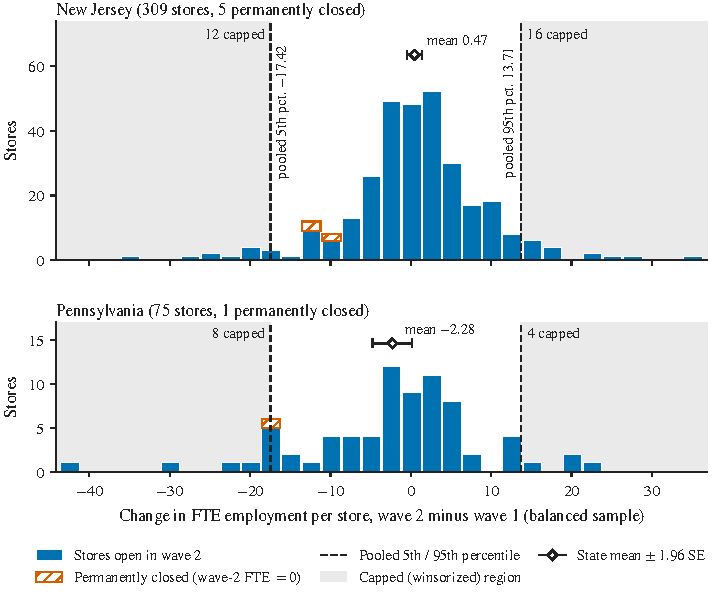
\includegraphics[width=0.85\textwidth]{figures/fig_dfte_dist.pdf}
\caption{Distribution of the store-level change in FTE employment between wave~1
(February--March 1992) and wave~2 (November--December 1992) on the balanced sample: New
Jersey (top, $\NBalNj$ stores) and Pennsylvania (bottom, $\NBalPa$ stores). Bars count
stores in 2.5-FTE bins; hatched segments are permanently closed stores, whose change is
$-$FTE$_1$. Dashed lines are the pooled 5th and 95th percentiles used by H2
($\HTwoQZeroFive$ and $\HTwoQNineFive$), computed over both states with closures included;
stores in the shaded tails are capped at the cutoff in the H2 estimate, and the printed
counts are the capped stores in each state and tail. The diamond and bar show the state's
unwinsorized mean change (row~4) with $\pm 1.96$ S1 standard errors, a sampling interval for
the mean, not a spread of the stores. A bin that straddles a cutoff is drawn whole. The
panels have their own y-axes, both starting at zero.}
\label{fig:dist}
\end{figure}

Figure~\ref{fig:dist} shows the store-level changes behind row~4. They are widely spread in
both states, with long tails on both sides. The pooled cutoffs are $\HTwoQZeroFive$ and
$\HTwoQNineFive$ FTE. Below the lower cutoff lie $\HTwoCappedLowNj$ New Jersey and
$\HTwoCappedLowPa$ Pennsylvania stores, $\HTwoCappedLowClosed$ of them a permanent closure
(in Pennsylvania); above the upper cutoff lie $\HTwoCappedHighNj$ New Jersey and
$\HTwoCappedHighPa$ Pennsylvania stores (permanent closures among them:
$\HTwoCappedHighClosed$).

Winsorized, the difference is $\HTwoWinsorized$ ($\HTwoWinsorizedSe$) against
$\HTwoUnwinsorized$ ($\HTwoUnwinsorizedSe$) unwinsorized on the same $\HTwoN$ stores, a
ratio of $\HTwoRatio$ (Table~\ref{tab:h2}, columns~1--2). The sign is unchanged and more than
half the magnitude is kept, so \textbf{H2 holds}.

The design anticipated that the permanent closures, whose change is minus their whole
first-wave workforce, might sit in the low tail and lift the New Jersey mean when capped.
On these data that is not what drives the result: $\HTwoCappedLowClosed$ closure is capped
(Table~\ref{tab:h2}), and with the closures left out of winsorization (secondary s1, column~3) the
difference is $\HTwoClosuresExcl$, a ratio of $\HTwoClosuresExclRatio$.

The stores capped in the low tail were large in the first wave: their mean FTE$_1$ is
$\HTwoFteOneCappedLow$, against $\HTwoFteOneBal$ on the balanced sample; the stores capped in
the high tail averaged $\HTwoFteOneCappedHigh$. The shrinkage comes mainly from capping the
declines of the Pennsylvania stores in the low tail (Table~\ref{tab:h2} gives the capped
counts by state and tail), which raises the Pennsylvania mean change. With few Pennsylvania
stores, a handful of them can move that mean (Section~\ref{sec:limitations}). Because the
narrowing comes from capping control-state stores, it says nothing about the heterogeneity
of New Jersey effects by store size that \citet{ropponen2010cic} reports, and his
changes-in-changes estimate answers a different question from this check.

\paragraph{What H2 does and does not show.} H2 shows that the balanced-sample estimate is
not produced by the parts of the store-level changes beyond the 5th and 95th percentiles:
winsorization caps those stores at the cutoffs rather than removing them, and with their
changes capped the difference keeps $\HTwoRatio$ of its size. It does not answer the measurement-error critique of
\citet{neumark1995payroll}, who state that the greater variability of the survey's
employment changes is not driven by one or two outliers. Winsorizing the tails leaves the
variability in the middle of the distribution untouched, and with it any error it
carries. This check does not show that the
estimate survives their critique.

\subsection{The Neumark--Wascher sample rule}

Under the rule of \citet{neumark1995payroll}, the balanced sample without the permanently
closed stores ($\NwRuleN$ stores) and chain and ownership controls, the New Jersey
coefficient is $\NwRuleDid$ ($\NwRuleDidSe$; HC1 $\NwRuleDidSeHcOne$), with unadjusted mean
changes of $\NwRuleChgNj$ in New Jersey and $\NwRuleChgPa$ in Pennsylvania
(Table~\ref{tab:h2}, column~4). Neumark and Wascher report 2.78 for this rule, with changes of
$+0.66$ and $-2.1$. The numbers agree, but their sample size is not recorded in our sources,
so we do not claim that the samples are the same. This is a report-only secondary. It
concerns their re-estimate on the survey data, not their payroll data, and it bears neither
on the payroll evidence nor on Card and Krueger's reply to it.

\subsection{A descriptive comparison, not a test of parallel trends}

The identifying assumption is that, absent the rise, mean FTE employment at the New Jersey
stores would have changed as much as at the Pennsylvania stores. With two waves it cannot be
tested, and no planned run could contradict it. Before the rise, New Jersey stores were
smaller: the first-wave level difference is $\LevelGapWOne$ ($\LevelGapWOneSe$) FTE, and the
second-wave difference is $\LevelGapWTwo$ ($\LevelGapWTwoSe$).

The plan includes one descriptive comparison. Of the 73 New Jersey stores that already paid \$5.00 or more in the first wave, the
$\PlaceboHiwageN$ with first-wave employment data changed by $\PlaceboHiwageNj$ under the row-3
rules, against $\DidFtePa$ in Pennsylvania, a difference of $\PlaceboHiwage$
($\PlaceboHiwageSe$); on the balanced sample it is $\PlaceboHiwageRFour$
($\PlaceboHiwageRFourSe$). We report this as a description only and do not cite it as
support for parallel trends, for two reasons fixed before the run. Its answer was already
known from the published table (a change of $-2.04$ for these stores against $-2.16$ in
Pennsylvania), so it could not surprise us. And stores paying between \$5.00 and \$5.04 were
bound by the new \$5.05 minimum, so the group is not untreated.

\section{Inference with one treated and one control state}
\label{sec:inference}

Treatment in this design varies only between two states. The track rules of our crew call
for standard errors clustered at the level at which treatment varies; with two clusters that
is impossible. Every standard error in this paper, as in the original, is a cross-store
sampling error: it measures how much the state means would vary if different stores had been
surveyed, and it ignores any shock between the waves that hit one state's restaurants as a
whole. \citet{conley2011inference} show that with a small number of policy changes
conventional difference-in-differences inference can be misleading, and that the
treatment-effect estimator should not be treated as consistent. We therefore report the
standard errors only to compare them with the published ones (deviation D1,
Section~\ref{sec:deviations}). We do not present the published $t$ statistic of 2.03, or any
$t$ statistic of ours, as design-based evidence that the effect differs from zero, and H2 is
judged on point estimates only. The store-clustered standard errors of the stacked regression
cluster at the store, not at the level of treatment; they address only the repeated
observation of a store across waves (deviation D2).

\section{Limitations}
\label{sec:limitations}

\begin{itemize}
  \item \textbf{Data release.} The public file accompanies \emph{Myth and Measurement}, not
        the 1994 article. The row-3 gap and the Table~4 dependent mean could reflect a
        different release, an inconsistency in the published tables, or something else; our
        data cannot distinguish these.
  \item \textbf{Standard errors.} S1 is our reconstruction. It reproduces the balanced-sample
        errors, where it reduces to the obvious formula, and not the row-3 errors. We do not
        know how Card and Krueger computed the row-3 standard errors.
  \item \textbf{Not a blind test.} The Table~4 sample size was observed at data preparation;
        the published values of every target, an earlier replication's 2.75, and the
        published results of the authors' and Neumark and Wascher's robustness checks were
        known before the hypotheses were fixed. The process rules out search over
        specifications within this study, not prior knowledge.
  \item \textbf{H2 covers the tails only.} The 5th and 95th percentiles are one fixed choice;
        other cutoffs, trimming or distributional estimators were not run and would be
        exploratory. The balanced Pennsylvania sample has only $\NBalPa$ stores, so a pooled
        tail holds few of them and one store can move the Pennsylvania mean. Measurement
        error in the middle of the distribution is not addressed.
  \item \textbf{Identification.} Parallel trends is maintained, not validated. The descriptive
        high-wage comparison is not a test of it.
  \item \textbf{Inference.} With two states, no standard error here supports a claim of
        statistical significance about the policy (Section~\ref{sec:inference}).
  \item \textbf{Scope.} The payroll data of \citet{neumark1995payroll} and the BLS ES-202 data
        of \citet{card1998reanalysis} are not public. This paper says nothing about which of
        those sources is right, or about minimum-wage effects beyond these restaurants and
        this period.
  \item \textbf{Sources read only in part.} The full texts of \citet{neumark2000comment},
        \citet{card2000reply}, \citet{ropponen2011reconciling} and \citet{ropponen2014note}
        were not available to us, and \citet{conley2011inference} was read from its
        abstract. Of \citet{neumark1995payroll} the abstract and pages~1--10 were read
        and the rest only keyword-searched; of \citet{card1998reanalysis} the abstract,
        introduction and Section~I.A were read. We cite these for no more than what we
        could read.
\end{itemize}

\section{Deviations and disclosures}
\label{sec:deviations}

\paragraph{Deviations from the track rules, approved at the design gate.}
\begin{itemize}
  \item \textbf{D1.} Standard errors are not clustered at the level of treatment, because
        there are only two states. They are cross-store sampling errors, reported only for
        comparison with the published ones; no hypothesis is judged on significance.
  \item \textbf{D2.} The store-clustered standard errors of the stacked regression cluster at
        the store, not the treatment level, and are reported only.
\end{itemize}

\paragraph{Deviations in the analysis.} None. Every analysis run in the approved plan was
executed once, on the reviewed code, in the planned order; none was repeated or replaced,
and no sample rule, FTE definition, standard-error method or decision rule was changed after
any result was seen. The fixes that followed the code review (Section~\ref{sec:impl}) were
made before any analysis run. The synthetic-data test, a data-preparation run, was rerun
once after the test script was extended; its first record is archived.

\paragraph{Order of the design gate and the code review.} The plan's task for the design
gate said it would be requested after the design and code reviews. It was requested after
the design review only and approved by the human author on 2026-11-19 at 06:52 UTC, before
the analysis code existed. The code was then written, tested on synthetic data and reviewed
(the code review is dated 07:06 UTC), all before any analysis run. The protocol's binding
rule, that the design gate be approved and the latest code review be free of critical and
major findings before any analysis run, was met; the order stated in the task was not. No
estimate is affected.

\paragraph{Unplanned runs.} Four analysis-kind runs that are not in the plan built the
tables and the figure after the results gate: \texttt{pub-values}, \texttt{tab-replication},
\texttt{tab-h2} and \texttt{fig-dfte-dist}. They read only logged metrics, the logged
store file and the crew's transcription of the published tables, and compute no new
estimate.

\paragraph{Corrections to the record after the results review.} The Reviewer's first results
review found that the crew's notes called the row-3 gap a rounding difference, explained the
passing difference-SE target backwards (as following from the low New Jersey error), and set
rows~1--2 against row~3 as if they could disagree; the second found that the notes said
Table~4 matched at every digit although its dependent mean does not. The notes and claim
texts were corrected before the results gate. No estimate changed; the corrected wording is
the one used here.

\paragraph{Presentation.} The published values in
Table~\ref{tab:replication} are parsed from the crew's transcription of the original tables,
and the script checks the fifteen H1 targets against the values the verdict used. The
absolute differences shown for report-only cells are a comparison added at this stage; no
tolerance is applied to them. An unplanned comparison noted in the crew's run notes, the
published and replicated standard errors of the high-wage New Jersey change, is not reported
here because it has no logged claim.

\paragraph{Framing.} The plan first described H2 as an implementation of Neumark and
Wascher's measurement-error critique. The Reviewer pointed out, before the design gate, that
their own text rules out reading a tail-only check that way; the hypothesis was relabelled as
a tail-only check, and that is the reading used here. No estimate outside the plan was
computed, so the paper has no exploratory section.

\section{Conclusion}

From the authors' public file and their own SAS rules, the balanced-sample
difference-in-differences of \citet{card1994minimum}, its within-state changes and standard
errors, and the Table~4 column~(i) regression on 357 stores are reproduced. The headline
row~3 estimate is within our pre-registered tolerance but not at published precision; the
gap sits in the unbalanced wave means, is not rounding, and has no source we could identify.
For its standard errors the verdict is ``point reproduced; SE construction not
identified'': we could not identify how they were computed. Capping the most extreme
store-level changes at the pooled 5th and 95th percentiles leaves the balanced-sample
estimate at $\HTwoRatio$ of its size, so the estimate is not driven by the parts of the
changes beyond the cutoffs; that leaves Neumark and Wascher's broader concern about measurement error, and
the question of what one treated and one control state can establish, where they were.

\section*{AI-use statement}

This paper was drafted by a crew of AI research-assistant agents
(Free-Research-Crew, protocol v0.1) under the direction of the human author, Bryce Wang.
He approved the research question (2026-11-19, 01:17 UTC), the design (2026-11-19,
06:52 UTC) and the results (2026-11-19, 08:01 UTC) at three human gates, each in chat after
reading the Reviewer's verdict and kill argument. The manuscript itself is subject to a
fourth, the submission gate. He takes responsibility for the paper's content.

\begin{itemize}
  \item \textbf{Roles and models.} Every crew role ran on Anthropic Claude through Claude
        Code. The PI role was the main Claude Code session. The Scout, Data RA, Designer,
        Econometrician, Figures RA, Reviewer, Replicator and Writer ran as agents launched
        from that session. The review records name the model as
        \texttt{claude-opus-5-5}. The PI's brief to each agent was archived in
        \texttt{briefs/} from the question stage on, beginning with the Scout's first brief
        (2026-11-18, 16:28 UTC).
  \item \textbf{Review.} The Reviewer ran 3 rounds on the research question, 1 on the
        design, 1 on the code, 2 on the results and 2 on the paper (round~1: revise; round~2: pass with minor
        findings open). No separate
        literature round was held. The code review passed before any analysis run; it came after the design gate, not
        before it as the plan's task said (Section~\ref{sec:deviations}). The
        Reviewer's independence level was \emph{fresh-context}: a new context in every
        round, with the same model family as the other roles. The human author chose this
        over a cross-family reviewer. The final round of each stage passed with minor
        findings still open, all answered before the next gate:
        \begin{itemize}
          \item question round~3 (three findings), answered in the design;
          \item design round~1 (six findings), answered in the plan before the design gate;
          \item code round~1 (three findings), fixed before any analysis run;
          \item results round~2 (two findings), answered in the run notes and claims before
                the results gate;
          \item paper round~2 (four findings), answered in this version: an attribution of
                the H2 narrowing to particular stores that no logged run supports was
                removed, the findings of the two results reviews are now assigned to the
                right round, ``every number'' was narrowed to ``every result number'', and
                this item was completed.
        \end{itemize}
  \item \textbf{Findings accepted over the Reviewer's objection.} None.
  \item \textbf{Evidence.} Every result number in the text and tables is a macro generated
        from the metrics of a logged run, or is written by a logged table script from run
        metrics. The numbers typed by hand are of three kinds:
        \begin{itemize}
          \item design facts fixed in the plan before any analysis run: the minimum wages,
                the survey dates, the targets, the 0.05 tolerance, the 5th and 95th
                percentiles, the store and closure counts checked at data preparation, and
                the Reviewer's pre-run calculation for the row-3 New Jersey standard error;
          \item published or source facts, quoted as the Scout's source notes record them,
                and arithmetic on published entries only;
          \item process facts: dates, review-round counts and the file size of the data
                archive.
        \end{itemize}
        Every citation was checked against its source by the Scout. Of the 12 sources cited, 5
        were read in full text (the original article's tables from page images), 2 in part
        (\citet{neumark1995payroll}: abstract and pp.~1--10, the rest keyword-searched;
        \citet{card1998reanalysis}: abstract, introduction and Section~I.A), 3 from the
        abstract only and 2 by resolving their DOI; the paper cites each for no more than
        was read. The full workspace is public at
        \url{https://github.com/brycewang-stanford/Free-Research-Crew/tree/main/gallery/ss-card-krueger}.
        It contains the plan, the run ledger and notes, the code, the data manifest, every
        review, the archived briefs and the source notes.
  \item \textbf{Replication.} Passed. The Replicator's clean rerun, recorded in
        \texttt{replication.json} (2026-11-19, 12:29 UTC), copied the workspace, deleted every recorded output, fetched the data
        again rather than reusing it, and re-executed all 15 logged runs in a fresh
        environment built only from \texttt{code/requirements.txt}. All 15 reproduced
        their logged metrics within a relative tolerance of $10^{-6}$. The steps are in
        \texttt{REPLICATION.md}.
\end{itemize}


% A copy of plainnat.bst that keeps the case of titles as written in refs.bib.
\bibliographystyle{plainnat-keepcase}
\bibliography{../refs}

\end{document}
